\chapter{Introduction}
\minitoc
\section{Artificial Intelligence foundations}

Machine Learning, the computer science subdomain dedicated to building and studying computer systems that automatically improve with experience, is at the very core of the recent advances in Artificial Intelligence. Finding its roots in statistical analysis, it has been widely studied over the past thirty years from algorithmic and mathematical perspectives, giving rise to a new discipline, computational learning theory. With the availability of massive amounts of data and computing power at low price, the last two decades have witnessed a growing interest in  real-world applications of the domain. This interest is even stronger since 2012, with the remarkable success of of AlexNet~\citep{krizhevsky2012imagenet} on the ImageNet challenge~\citep{imagenet_cvpr09}, using neural networks with several layers. The era of Deep Learning started then, with  unexpected achievements in several domains: generative modeling~\citep{goodfellow2014generative}, natural language processing~\citep{vaswani2017attention}, etc. The success of Deep Learning (artificial neural networks with a large number of layers) can be explained by the conjunction of the following factors: 

%Machine learning can be defined with the following question: ``How can we build computer systems that automatically improve with experience, and what are the fundamental laws that govern  all learning processes?''. For instance, credit scoring are computed rules that are learnt from previous defaulting consumers. Machine Learning have been widely studied for the $30$ past years using advanced statistical tools and taking profits of more and more powerful computers.  The last $10$ years have seen an exponentially increasing public interest for machine learning systems. Firstly, this incredible growth of interest to AI is also linked to the availability of huge amounts of data at low price, the so-called ``Big Data'' era.  Secondly, the advent of Deep Learning, i.e. Machine Learning using Artificial Neural Networks with a lot of layers, came with the extraordinary success of AlexNet~\citep{krizhevsky2012imagenet} on the ImageNet challenge~\citep{imagenet_cvpr09} in 2012. Since, exceptional progresses were made in generative modeling~\citep{goodfellow2014generative}, natural language processing~\citep{vaswani2017attention}, etc. Machine learning has become the most active research fields in Artificial Intelligence. Therefore the number of industrial application has also exploded. The recent renewal in Machine Learning is due to the conjunction of many factors:
\begin{itemize}
    \item \textbf{Availability of data:} the amount and the cost of data have largely decreased since the emergence of web platforms, and tools for large-scale data management.
    \item \textbf{Computational power:} new specialised hardware architectures such as GPUs and TPUs allow faster and larger training algorithms.
    \item \textbf{Algorithmic scalability:} algorithms are scalable to large models (Distributed Computing, etc.) and large number of data (Stochastic Gradient Descent~\citep{bottou2010large}, etc.)
    \item \textbf{Open Source projects:} Large projects in Machine Learning are nowadays open-sourced (TensorFlow~\citep{abadi2016deep}, PyTorch~\citep{paszke2017automatic}, Scikit Learn~\citep{sklearn}, etc.) stimulating the emergence of large communities.
\end{itemize}

It is worth noting here that Artificial Intelligence, as a scientific domain, exists since early 20th century. Protean in nature, it encompasses several notions and fields, beyond Machine Learning, and Deep Learning.  Its birth is inseparable from the development of computer science. The first efficient computer was built by Charles Babbage and ran Ada Lovelace's algorithm.  Computer Science was formalized and theoretized in the Church-Turing thesis~\citep{turing1950computing}, which defines the notion of computability, i.e. functions are computable if they can be out as a list of predefined instructions to be followed. Such instructions are called algorithms. Artificial Intelligence, or at the least the term,  was  ``officially founded'' as a research field in 1956 at the Dartmouth Workshop~\citep{mccarthy2006proposal}, organized by Marvin Minsky, John McCarthy, Claude Shannon and Nathan Rochester. During this conference, the term ``Artificial intelligence'' was proposed and adopted by the community of researchers. Since then, the field has oscillated between hype and disappointment, with no less than two major period of disinterest  as the AI winters. This thesis is clearly developed during the third hype's period, but we keep in mind the very enlightening  history of the discipline.  

%Following this conference and thanks to (military) fundings, substantial advances in the field were made in problem solving and natural language processing. However the results, being far from meeting the funders' expectations, the domain   entered in a first ``AI winter'' during late sixties and the seventies. The second wave of AI occured thanks to the fundamental limits of symbolic AI and expert systems that allow focus on new designs of Artificial Neural Networks thanks to the algorithm of backpropagation~\citep{rumelhart1985learning} and the first well performing convolutional networks~\citep{lecun1995convolutional}. In the 1980s, theoretical analysis of machine learning also appeared with the theory of learning~\citep{valiant1984theory,vapnik1998} with the first generalization bounds on learning algorithms. Until the success of Deep Learning, Support Vector Machines~\citep{vapnik1998} and kernel methods~\citep{vert2004primer} were the most popular methods in Learning problems.


% TALK ABOUT CYBERNETICS

\section{Risks with Learning Systems}
% The idea of building artificial intelligence dates back to the first automatons that dates back to Ancient Egypt and Greece mythology. At the time, automatons were movable statue as Talos' one in Crete. Artificial Intelligence relies on the idea that human reasoning can be automatized, e.g. building a machine that can replicate human reasoning without external intervention. The study of automatized reasoning has a long stand history, and was the research subject of many mathematicians or philosophers. QUOTE A BIT
% A ENLEVER PE





\subsection{Common Threats}
Cybersecurity is at the core of computer science. Cryptography has been one of the hottest topics during the last thirty years. Despite their performances, learning systems are subject to many types of vulnerabilities and, by their popularity, are then prone to malicious attacks. Probably, the most known vulnerability that got public attention is privacy. While the amount of available data is exponentially growing, recovering identities by crossing datasets is easier when data are not protected. As it was exhibited in the de-anonymization of the Netflix 1M\$ prize dataset~\citep{narayanan2008robust}, hiding identities in datasets is not sufficient to protect the privacy data. Computer scientists have then intensified their effort so as to propose ways to protect data, leading to the emergence to what is considered as a gold standard for data protection: Differential Privacy~\citep{dwork2008differential}. It barely consists in adding noise to data to make them unrecoverable without too much deteriorating the their utility. It is appealing because it comes with strong theoretical guarantees, while being simple to manipulate,  allowing to tradeoff between the degree of privacy through noise injection and the quality of the information one can infer from the data.  Common privacy attacks are:
\begin{itemize}

    \item  \textbf{Model stealing~\citep{tramer2016stealing}:} An attacker aims at stealing the parameters of a given model.
    \item \textbf{Membership inference~\citep{shokri2017membership}:} Inferring whether a data sample was present or not in a training set. 

\end{itemize}
    

Consequently to privacy threats, European authorities conceived the GDPR (General Data Protection Regulation)\footnote{\url{https://eur-lex.europa.eu/eli/reg/2016/679/oj}}, adopted in 2016, which defines new rules on the use of data and on privacy. Today, GDPR is part of any data management plan of private companies. 
%Indeed, the fine for a company not respecting this law can be up to $4\%$ of the revenues of the company. To comply with this new regulation, companies and government must respect privacy in the implementation of any system with regards to the data they use.  While the initial aim of such a law was to discourage multinational companies using personal data, these companies has adapted easier than smaller ones thanks to the budget they could allocate for respecting GDPR. To counter this,
As an update of the GDPR, a second law proposition regarding data sharing from public and private companies has been introduced by the European Commission on The Governance of Data\footnote{\url{https://eur-lex.europa.eu/legal-content/EN/TXT/?uri=CELEX\%3A52020PC0767}} in 2020.

    
    
Another type of vulnerability in Machine Learning is model failure. A malicious user, by modifying either the model or the data, can make it performs very poorly. The most known attacks aiming at model failures are:
\begin{itemize}
    \item \textbf{Data poisoning attacks~\citep{kearns1993learning}:} changing some data in the training set so that the model performs very poorly on the hold-out set. 
    \item \textbf{Evasion attacks~\citep{biggio2013evasion,Szegedy2013IntriguingPO}}: small imperceptible perturbations at inference time. We will refer them to \emph{``adversarial attacks''}.
\end{itemize}
    
Known and gaining interest in academia, these threats are not very known by most of the companies~\cite{kumar2020adversarial}. More importantly, such vulnerabilities  hinder the use of state of the art models in critical systems (autonomous vehicles, healthcare, etc.). In the manuscript we will focus on adversarial attacks.  We introduce this threat more in details in the next paragraph.

\begin{tcolorbox}[title=References to adversarial examples in European Commission in law proposal on Artificial Intelligence systems]
\label{ref:adversarial_law}
As part of the introduction: \textit{``Cybersecurity plays a crucial role in ensuring that AI systems are resilient against attempts to alter their use, behaviour, performance or compromise their security properties by malicious third parties exploiting the system’s vulnerabilities. Cyberattacks against AI systems can leverage AI specific assets, such as training data sets (e.g. data poisoning) or trained models (e.g. adversarial attacks), or exploit vulnerabilities in the AI system’s digital assets or the underlying ICT infrastructure. To ensure a level of cybersecurity appropriate to the risks, suitable measures should therefore be taken by the providers of high-risk AI systems, also taking into account as appropriate the underlying ICT infrastructure.''}

\medskip
Title III (High risk AI systems), Chapter II (Requirements for high risk AI system), Article 14.52 (Human oversight): \textit{``High-risk AI systems shall be resilient as regards attempts by unauthorised third parties to alter their use or performance by exploiting the system vulnerabilities.
The technical solutions aimed at ensuring the cybersecurity of high-risk AI systems shall be appropriate to the relevant circumstances and the risks.
The technical solutions to address AI specific vulnerabilities shall include, where appropriate, measures to prevent and control for attacks trying to manipulate the training dataset (‘data poisoning’), inputs designed to cause the model to make a mistake (‘adversarial examples’), or model flaws.''}
\end{tcolorbox}
\medskip
A first regulation text on Artificial Intelligence\footnote{\url{https://eur-lex.europa.eu/legal-content/EN/TXT/?uri=CELEX\%3A52021PC0206}} systems was proposed by the European commission in April 2021. This text includes a large section dedicated to ``High Risk AI''. High risk AI is referred to any autonomous system than can endanger human lives.  This text aims at dealing with many threats in Learning Systems. Two direct references are made to adversarial attacks, underlying the need for companies to deal with them. The difficulty is to unify and create precise rules in a domain where results and certificates are mostly empirical. As mentioned earlier, it is known that robust models are often less performing and can make autonomous systems unusable in real world scenarii. Thus, this text is a first step towards a unified regulation on autonomous systems but might miss precise requirements for models to be used in production.


\subsection{Adversarial attacks against Machine Learning Systems}

Despite the recent gain of interest in studying adversarial attacks in Machine Learning, the problematic exists however for a while and takes its source in SPAM classification where adversaries were spammers whose goal was to evade from the taken decision\footnote{\cite{dalvi2004adversarial} showed that linear classifiers used in spam classification could be fooled by simple ``evasion attacks'' as spammers inserted ``good words'' into their spam emails.}.

With the recent success of Deep Learning algorithms, in particular in computer vision, several authors~\citep{biggio2013evasion,Szegedy2013IntriguingPO} have  highlighted their vulnerability to adversarial attacks. Adversarial attacks in this case are widely understood as ``imperceptible'' perturbations of an image, i.e. slight changes in the pixels, so that this image remains unchanged from human sights. This characteristic might be surprising but is actually a severe curb in applying state-of-the-art deep learning methods in critical systems. There are number of issues that makes difficult building and evaluating robust models for real life applications:
\begin{enumerate}
    \item The notion of imperceptibility is not well understood: numerically measuring human perception is still an open problem. Hence, detecting the change of perception due to adversarial attacks is an ill-posed problem. Most of the  research in the domain focused on pixel-wise perturbations (e.g. $\ell_p$ norms), while real world threats would be crafted by inserting some misleading objects in the environment (e.g. patches~\citep{brown2017adversarial}, T-shirts~\citep{xu2020adversarial}, textures~\citep{wiyatno2019physical},etc.).
    \item Robustness is often empirically measured: there exist only a few methods with formal guarantees on the robustness and these guarantees are often loose. Robustness is usually measured on a set of possible attacks and not all possible perturbations are spanned by these attacks, leaving rooms for potential blind spots.
    \item There exists a trade-off between robustness and accuracy. Most models that are robust suffer from a performance drop on natural data. For instance, a robustly trained robot will perform much lower on natural tasks than an accurate non-robust robot. That makes robust models unusable in real world applications~\citep{lechner2021adversarial}. 
\end{enumerate}

%ENLEVER CE QU Il Y A EN DESSOUS ?

%The substantial gap between academic research on adversarial attacks and ``real world'' attacks is difficult to bridge and it is one of the reasons authorities are reluctant authorizing autonomous systems as driver-free cars~\citep{eykholt2018robust}, automated face recognition as biometry checks~\citep{dong2019efficient}, etc.  The proposal from European Commission on AI highlights the risk of Adversarial Examples on algorithms  in production. 



\section{Adversarial Classification in Machine Learning}

In this manuscript, we will focus on the task of classification in Machine Learning. The purpose of this task is to ``learn'' how to classify some input $x$ into some label(s). The input can be an image, a text, an audio, etc. For instance, in computer vision, a known dataset is ImageNet where the goal is to learn how to classify high quality images into $1000$ labels~\citep{imagenet_cvpr09}. In natural language processing, the IMDB Movie Review Sentiment Classification dataset~\citep{maas-EtAl:2011:ACL-HLT2011} aims at classifying positive or negative sentiments from movie reviews. To learn a classifier, the task is often supervised, i.e, we have access to labeled inputs, which constitutes the so-called training set. To assess the quality of the learnt model, we evaluate it on other images that constitute the test set.

\subsection{A Learning Approach for Classification}
From now, we will assume that the inputs are in some space $\XX$ and the labels form a set $\mathcal{Y}:=\{1,\dots,K\}$. To learn an adequate classification model, we denote $\{(x_1,y_1),\dots,(x_\numsamples,y_\numsamples)\}$ the $\numsamples$ elements of $\XX\times\YY$ forming the training set. We furthermore assume that these inputs are independent and identically distributed (i.i.d.) from some distribution $\PP$ on $\XX\times\YY$. The aim is now to learn a function/hypothesis from these samples $h:\XX\to\YY$ to classify an input $x$ with a label $y$. To assess the quality of a classifier, the metric of interest is often the misclassification rate of the model, or the $0/1$ loss risk, and it is defined as:
\begin{align*}
\risk_{0/1}(h):=\PP(h(x)\neq y) = \EE_{(x,y)\sim\PP}\left[\mathbf{1}_{h(x)\neq y}\right]
\end{align*}
The optimal classifier, minimizing the standard risk is called the Bayes optimal classifier and is defined as $h(x) = \argmaxB_k\PP(y=k\mid x)$.
As the sampling distribution $\PP$ is usually unknown, the optimal Bayes classifier is also unknown. The accuracy is often empirically evaluated on a test set $\{(x'_1,y'_1),\dots,(x'_M,y'_M)\}$ independent from the training set and i.i.d. sampled from $\PP$.  To find this classifier $h$, we learn a function $\mathbf{f}:\XX\to\mathbb{R}^K$ returning scores, or logits, $(f_1(x),\dots,f_K(x))$ corresponding to each label. Then $h$ is set to $h(x)=\argmaxB_k f_k(x)$. The function $\mathbf{f}$ is usually learned by minimizing the empirical risk for a certain convenient loss function $\loss$ over some class of functions $\mathcal{H}$.
\begin{align*}
\inf_{\mathbf{f}\in\mathcal{H}}\riskemp_{\numsamples}(\mathbf{f}):= \frac{1}{\numsamples}\sum_{i=1}^\numsamples \loss(\mathbf{f}(x_i),y_i).
\end{align*}

This problem is called Empirical Risk Minimization (ERM). The theory of this problem has been widely studied and is well understood. It is often argued that there is a tradeoff on the ``size'' of $\mathcal{H}$: having a too small $\mathcal{H}$ may lead to underfitting, i.e. not enough parameters to describe the optimal possible function while a too large $\mathcal{H}$ may lead to overfitting, i.e. fitting too much training data. We often talk about bias-variance tradeoff (see Figure~\ref{fig:tradeoff_bias_accuracy}). A penalty term $\Omega_{\mathcal{H}}(\mathbf{f})$ can also be added to the ERM objective to prevent from overfitting. This tradeoff was recently questioned by the double descent~\citep{belkin2019reconciling} phenomenon where overparametrized (i.e. number of parameters largely over the number of training samples) regimes lower the risk.
\begin{figure}
    \centering
    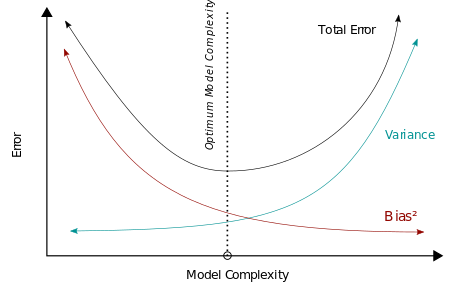
\includegraphics[width=0.5\textwidth]{Images/tradeoff_bias_variance.png}
    \caption{Bias-Variance tradeoff. A model with low complexity will have a low variance but an high bias. A model with high complexity will have a low bias but an high variance.}
    \label{fig:tradeoff_bias_accuracy}
\end{figure}
\begin{tcolorbox}
The presence of adversaries in classification questions the knowledge we have in standard statistical learning. Indeed most standard results do not hold in presence of adversaries, hence, opening a new research area dedicated to studying and understanding the classification problem in presence of adversarial attacks, and more importantly, deepens our understanding of  machine learning/deep learning in high dimensional regimes.
\end{tcolorbox}


\subsection{Classification in Presence of Adversarial Attacks}

Though a model can be very well performing on natural samples, small perturbations of these natural samples can lead to unexpected and critical behaviours of classification models~\citep{biggio2013evasion,Szegedy2013IntriguingPO}. To formalize that, we will assume the existence of a ``perception'' distance $d:\XX^2\to\mathbb{R}$ such that a perturbation $x'$ of an input $x$ remains imperceptible if $d(x,x')\leq \varepsilon$ for some constant $\varepsilon\geq0$. This ``perception'' distance is difficult to define in practice. For images, the $\lVert\cdot\rVert_\infty$ distance over pixels is often used, but is not able to capture all imperceptible perturbations.  This choice is purely arbitrary: for instance, we will highlight in the manuscript that $\lVert\cdot\rVert_2$ perturbations can also be imperceptible while having a large $\lVert\cdot\rVert_\infty$. Image classification algorithms are also vulnerable to geometric perturbations, i.e. rotations and translations~\citep{kanbak2018geometric,engstrom2019exploring}.

Therefore, the goal of an attacker is to craft an adversarial input $x'$ from an input $x$ that is imperceptible , i.e. $d(x,x')\leq \varepsilon$ and misclassifies the input, i.e. $h(x')\neq y$. Such a sample $x'$ is called an adversarial attack. The used criterion cannot be the misclassification rate anymore, we need to take into account the possible presence of an adversary that maliciously perturbs the input. We then define the robust/adversarial misclassification rate or robust/adversarial $0/1$ loss risk: 
\begin{align*}
\risk_{0/1}^{\varepsilon}(h)&:=\PP_{(x,y)}(\exists x'\in\XX\text{ s.t. } d(x,x')\leq \varepsilon \text{ and } h(x')\neq y)\\
&= \EE_{(x,y)\sim\PP}\left[\sup_{x'\in\XX\text{ s.t. } d(x,x')\leq \varepsilon}\mathbf{1}_{h(x')\neq y}\right]
\end{align*}
Akin standard risk minimization, we aim to learn a function $\mathbf{f}:\mathcal{X}\to\mathbb{R}^K$ such that $h(x)=\argmaxB_k f_k(x)$. Usually in adversarial classification we aim at solving the following optimization problem, that we will call adversarial empirical risk minimization:
\begin{align*}
\inf_{\mathbf{f}\in\mathcal{H}}\riskemp^\varepsilon_{\numsamples}(\mathbf{f}):= \frac{1}{\numsamples}\sum_{i=1}^\numsamples\sup_{x'\in\XX\text{ s.t. } d(x,x')\leq \varepsilon} \loss(\mathbf{f}(x_i),y_i).
\end{align*}
This problem is more challenging to tackle than the standard risk minimization  since it involves a hard inner supremum problem~\citep{madry2018towards}. Guarantees in the adversarial setting are therefore difficult to obtain both in terms of convergence and statistical guarantees. The usual technique to solve this problem is called Adversarial Training~\citep{goodfellow2014explaining,madry2018towards}. It consists in alternating inner and outer optimization problems. Such a technique improves in practice adversarial robustness but lacks theoretical guarantees. So far, most results and advances in understanding and harnessing adversarial attacks are empirical~\citep{ilyas2019adversarial,rice2020overfitting}, leaving many theoretical and practical questions open.  Moreover, robust models suffer from a performance drop and vulnerablity of models is currently still very high (see Table~\ref{table:sota-cifar}), which leaves room for substantial improvements.

\begin{table}[ht]
    \centering
    \begin{tabular}{c|c|c|c}
       \textbf{Attacker}  &  \textbf{Paper reference} & \textbf{Standard Acc.} & \textbf{Robust Acc.}  \\ \hline
        None & \citep{ZagoruykoK16} & 94.78\% & 0\%\\
        $\ell_\infty (\varepsilon=8/255)$&  \citep{rebuffi2021fixing}& 89.48\% & 62.76\%\\
        $\ell_2 (\varepsilon=0.5)$&  \citep{rebuffi2021fixing}& 91.79\% & 78.80\%\\
    \end{tabular}
    \caption{State of the art accuracies on adversarial tasks on a WideResNet 28x10~\citep{ZagoruykoK16}. Results are reported from~\citep{croce2020robustbench}}
\label{table:sota-cifar}
\end{table}

\section{Outline and Contributions}
We will first introduce in Chapter~\ref{chap:background} the necessary  background regarding Machine Learning and Adversarial Examples. We will then analyze  adversarial attacks from three complementary points of view outlined as follows.
\subsection{A Game Theoretic Approach to Adversarial Attacks}

A line of research, following~\cite{pinot2020randomization}, to understand adversarial classification is to rely on game theory. In Chapter~\ref{chap:game},  we will build on this approach and define precisely the motivations for both the attacker and the classifier. We will cast it naturally as a zero sum game. We will in particular, study the problem  of the existence of equilibria. More precisely, we will answer the following open question.
\medskip
\begin{tcolorbox}[title=Question 1]
\textbf{What is the nature of equilibria in the adversarial examples game?}
\end{tcolorbox}
\medskip

In game theory, there are many types of equilibria. In this manuscript, we will focus on Stackelberg and Nash equilibria. We will show the existence of both when both the classifier and the attacker play randomized strategies. To reach such equilibria, the classifier will be random, and the attacker will move randomly the samples at a maximum distance of $\varepsilon$. Then, we will propose two different algorithms to compute the optimal randomized classifier in the case of a finite number of possible classifiers. We will finally propose a heuristic algorithm to train a mixture of neural networks and show experimentally the improvements we achieve over standard methods.

This work \textbf{Mixed Nash Equilibria in the Adversarial Examples Game} was published at ICML2021.



\subsection{Loss Consistency in Classification in Presence of an Adversary}
In standard classification, consistency with regards to $0/1$ loss is a desired property for the surrogate loss $\loss$ used to train the model. In short, a loss $\loss$ is said to be consistent if for every probability distribution, a sequence of classifiers $(f_n)$ that minimizes the risk associated with the loss $\loss$, it also minimizes the $0/1$ loss risk. Usually, in standard classification, the problem is simplified thanks to the notion of calibration. We will see that the question of consistency in the adversarial problem is much harder. 
\medskip
\begin{tcolorbox}[title=Question 2]
\textbf{Which losses are consistent with regards to the $0/1$ loss in the adversarial classification setting?}
\end{tcolorbox}
\medskip
We tackle this question by showing that usual convex losses are not calibrated for the adversarial classification loss. Hence this negative result emphasizes the difficulty of understanding the adversarial attack problem, and building provable defense mechanisms. 
\subsection{Building Certifiable Models}

The last problem we deal with in this manuscript is the implementation of robust certifiable models. In short, a classifier is said to be certifiable at an input $x$ at level $\varepsilon$ if one can ensure there exist no adversarial examples in the ball of radius $\varepsilon$. This problem is challenging since it is far from trivial to come up with non vacuous bounds that are exploitable in practice.
\medskip
\begin{tcolorbox}[title=Question 3]
\textbf{How to efficiently implement certifiable models with non-vacuous guarantees?}
\end{tcolorbox}
\medskip
To this end, we propose two methods that enforce Lipschitzness on the predictions of neural networks:
\begin{enumerate}
    \item The first one consists in noise injection. We show that by adding a noise on an input of a classifier, we are able to get guarantees on the decision up to some level $\varepsilon$. This work \textbf{Theoretical evidence for adversarial robustness through randomization} was published at NeurIPS2019.
    \item A second one consists in building contractive blocks in a ResNet architecture. This method draws its inspiration from the continuous flow interpretation of residual networks. More precisely, we show that using a gradient flow of a convex function, our network is $1$-Lipschitz. We then design such a function, showing empirically and theoretically the robustness benefits of this approach. 

\end{enumerate}

% \section{Other Works in Appendix}
\subsection{Additional Works}
Additionally to the works we present in the main document, we also present some other contributions we made during the thesis. These are deferred to the appendices. 

Regarding adversarial examples, we will present:
\begin{itemize}
    \item \textbf{Adversarial Attacks on Linear Contextual Bandits (see Appendix~\ref{paper:banditsattacks}):} we build provable attacks against online recommendation systems, namely Linear Contextual Bandits. This work was published at NeurIPS2020.
    \item \textbf{ROPUST: Improving Robustness through Fine-tuning with Photonic Processors and Synthetic Gradients (see Appendix~\ref{paper:ropust}):} we use an Optical Processor Unit over existing defenses to improve adversarial robustness. This work was published at a workshop on Adversarial Attacks at ICML2021.
\end{itemize}
We  published a paper in optimal transport named \textbf{Equitable and Optimal Transport with Multiple Agents (see Appendix~\ref{paper:eot})} where we introduce a way to deal with multiple costs in optimal transport by equitably partitioning transport among costs.
We also published many works in the field of evolutionary algorithms:
\begin{itemize}

    \item \textbf{Variance Reduction for Better Sampling in Continuous Domains (see Appendix~\ref{paper:rescaling})}: we show that, in one shot optimization, the optimal search distribution, used for the sampling, might be more peaked around the center of the distribution than the prior distribution modelling our uncertainty about the location of the optimum. This work was published at PPSN2020.
    \item \textbf{On averaging the best samples in evolutionary computation (see Appendix~\ref{paper:kbest}):}  we prove mathematically that a single parent leads to a sub-optimal simple regret in the case of the sphere function. We provide a theoretically-based selection rate that leads to better progress rates. This work was published at PPSN2020.
    \item \textbf{Asymptotic convergence rates for averaging strategies (see Appendix~\ref{paper:kbestgen}):} we extend the results from the previous papers to a wide class of functions including $C^3$ functions with unique optima. This work was published at FOGA2021.
    \item  \textbf{Black-Box Optimization Revisited: Improving Algorithm Selection Wizards through Massive Benchmarking (see Appendix~\ref{paper:benchmark}):} We propose a wide range of benchmarks integrated in Nevergrad~\citep{nevergrad} platform. This work was published in the journal TEVC.
    
\end{itemize}
% In addition to these works, we also add interest in adversarial attacks against online recommendation systems, namely Linear Contextual Bandits. We designed algorithms that provably fool in 

% We also published works in the field of Derivative Free Optimization FOLLOW